% this file is called up by thesis.tex
% content in this file will be fed into the main document

%: ----------------------- name of chapter  -------------------------
\chapter{Movement models}\label{movimento} % top level followed by section, subsection



%: ----------------------- contents from here ------------------------
%In Delay Tolerant Networks nodes are often spread throughout the network and end-to-end connections are hard to establish.

Connectivity on the Internet relies primarily on the wired links, which are continuously connected in end-to-end, low-delay paths between sources and destinations. Protocols adopted in wired networks achieve the best performances where connections are continuous, with short or constant delays and low error rates. This is not the case of mobile networks.
\\

MANETs have an infrastructure that suffers from intermittent connectivity and changes in topology that can be difficult or impossible to predict. One of the causes of these characteristics is node mobility. Nodes in MANETs are free to move randomly and such widely varying mobility characteristics are expected to have a significant impact on the performance of the routing protocols.
\\

To overcome wired networks protocols problems, DTNs use store-carry-forward strategies to transmit data from a source to a destination. These imply that a node physically delivers data to the destination moving from the source location. Replication techniques can be adopted to increase the delivery ratio, copying the carried data and giving it to other nodes following a different physical path. In M2MShare we saw that nodes movement is used to extend the search area for a requested file, delegation of unaccomplished tasks are made to servant nodes exploring different areas and frequencies of encounters between nodes are used to determine if a node would be a good servant to delegate a task to.
\\

It is easy to observe that in DTNs, movements of nodes are essential for the performance of the whole network, since they have a big impact on adopted routing protocol: the mobility of the nodes affects the number of average connected links, which in turn affect the performance of the routing algorithm.
So one important aspect to consider achieving a good level of realism in DTN simulations is to simulate movements of nodes inside the simulated world. 
\\

Movements of nodes can be captured in simulations using real movement traces or synthetic traces generated by a movement model. The abstraction level of synthetic movement models is variable, so are the ways used to gather real world movement traces. Real user traces can be acquired using only short-range connections between devices or by using GPS-capable devices carried by users.
\\

A movement model can be simple, considering only random nodes movements, independent from other nodes or from the scenario; or it can be complex enough to also consider the impact of human relationships over movement behaviour. The complexity and realism of movement models influence positions, speed values and encounters between nodes inside the simulated world. It is desirable that these parameters be generated as realistically as possible, to evaluate routing protocols performance in a simulated scenario as close as possible to the real one. The model should also be generic and configurable enough to be used in different scenarios.
\\

In this chapter we show characteristics and differences between synthetic and real-trace-derived models. We illustrate some movement models showing how these implement and describe the movement of nodes in the simulation. Each description is accompanied by a screenshot to give a visual representation of node movement in the model. We focus on the Working Day Movement Model and finally we explain why we chose it for our simulations.

\section{Real user traces \textit{vs} Synthetic models}
The most realistic user movement or contact patterns are the ones that happen in the real world. Therefore, several studies have focused on tracking user movement to be able to use the traces later for direct simulations or to learn more about which characteristics are common in real user behaviour. Real movement traces have usually been obtained by analysing WLAN access point logs \cite{Balachandran:2002:CUB:511399.511359} \cite{Ghosh:2006:PMP:1132983.1132993} \cite{Shaffer:2005:AMM:1104998.1105285} or using devices equipped with GPS modules carried by users \cite{Ashbrook:2002:LSL:862896.881068}. Contact traces have mostly been collected from real-world experiments where users have been carrying around Bluetooth devices tracking other devices within range \cite{Natarajan:2007:UUI:1762888.1762904}.
\\

When real trace are been obtained by analysing WLAN access point data, only certain areas have covered and so movements outside access points communication range are not recorded. Using GPS modules limits mobility recording only to outdoor movements. Contact traces, on the other hand, allow analysis of only frequency and number of contacts between users, without showing their spatial movements and movement patterns. Also, devices used to obtain real traces are not always carried by the users, are not necessarily always turned on, or with the GPS module active. Paper \cite{ImpactofHumanMobility} argues that the on/off times are an important characteristic of wireless users that needs to be taken into account.
\\

%There are some other problems about directly using the collected traces in simulations. 
Other issues arise when using directly traces collected in simulations. Real world traces are usually from very specific environments like university campuses areas. These traces are not so generic to be used to simulate movement in a different environment, like a centre of a city, because behaviour and movement patterns of studied people are different. Also, users mobility is often very low, while using the network, and one node only meets a small portion of all other nodes in the area resulting in an incomplete trace of users movements and contacts.
\\


\section{Random Walk}
The Random Walk movement model (RW) is one of the simplest mobility models available. In this model the simulation area is an open empty space where nodes move. Each node randomly chooses an angle and a speed and for the next interval it moves using these speed and direction values. The choice is made for every simulation instant. \figurename~\ref{fig:random_walk} illustrates a sample topography showing the movement of nodes for the Random Walk Mobility Model. The Random Walk model is a memoryless mobility model, because information about the previous status is not used for future decisions. 
\begin{figure}[htpb]
  \begin{center}
    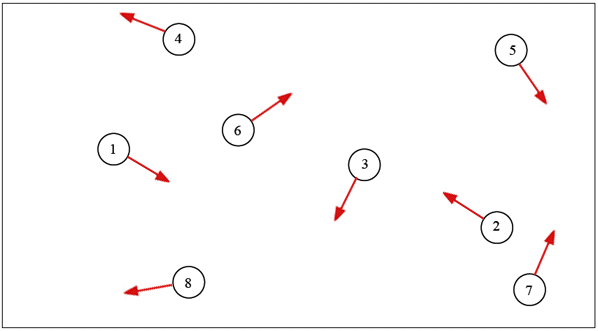
\includegraphics[scale=0.6]{4-movimento/img/random_walk.png}
    \caption{Example topography for Random Walk Movement Model}    
    \label{fig:random_walk}
  \end{center}
\end{figure}

\section{Random Waypoint}
The Random Waypoint movement model (RWP) is a generalization of RW and is one of the most frequently used models in mobility simulations. In this model every node chooses a random location within the simulation area and moves towards it at a random speed uniformly chosen from $(V_{min}, V_{max}]$, where $V_{min}$ is the minimum and $V_{max}$ is the maximum speed of the simulation. Like RW, in RWP the simulation area is an open empty space. When the node reaches its destination, it waits for a random amount of time and then repeats the previous steps (an example of topography for this model is shown in \figurename~\ref{fig:random_waypoint}). However, this model has a shortcoming as shown in
\cite{rwpharmful}: if the $V_{min}$ value is set to zero, as in the default implementation of the model, the simulation cannot reach a steady state and the average speed of nodes constantly decreases.

%This model has one shortcoming, however, shown in \cite{rwpharmful}, in that the simulation does not reach a steady state and average speed of nodes constantly decreases if the $V_{min}$ value is set to zero, as in the default implementation of the model. 
\begin{figure}[htpb]
  \begin{center}
    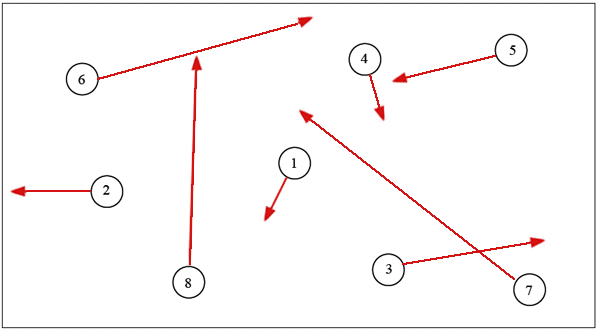
\includegraphics[scale=0.6]{4-movimento/img/random_waypoint.png}
    \caption{Example topography for Random Waypoint Movement Model}    
    \label{fig:random_waypoint}
  \end{center}
\end{figure}

\section{Random Map-Based Movement}
The simplest map-based mobility model is Random Map-Based Movement (MBM). Nodes adopting this model move randomly but always in the streets described on the map. This is done walking from one map node (i.e. an address on a street or a crossroad) to the other by always randomly selecting one of the directly connected map nodes (\figurename~\ref{fig:random_map}). Result of this behaviour is a random movement in which there are more contacts between nodes than in Random Walk model. This is due to the restriction of node movements in order to follow the streets described in the map.
\begin{figure}[htpb]
  \begin{center}
    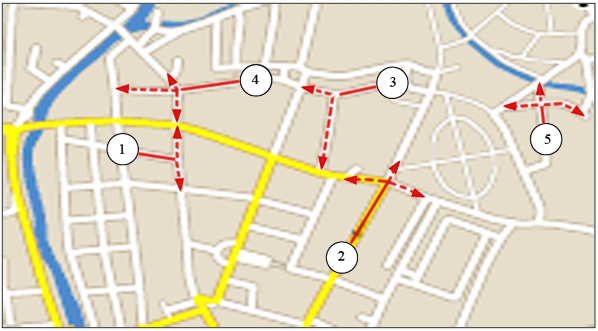
\includegraphics[scale=0.6]{4-movimento/img/random_map.png}
    \caption{Example topography for Random Map-Based Movement Model}    
    \label{fig:random_map}
  \end{center}
\end{figure}

\section{Shortest Path Map-Based Movement}
Shortest Path Map-Based Movement (SPMBM) is another mobility model that uses a map-described environment to restrict node movement. With this model, nodes choose their destination randomly inside the map, then calculate the shortest path to reach it and finally walk along this path, as shown in \figurename~\ref{fig:waypoint_map}. Dijkstra's algorithm is used to calculate the path. Destinations can be chosen in a totally random way or from a set of Points of Interests (POI). This can be useful to indicate interesting places like restaurants, monuments or shops. This model adds one level of realism, compared to MBM, since nodes don't move in a completely random way, but they have destinations and follow the best path to reach it, as most of humans would do.
\begin{figure}[htpb]
  \begin{center}
    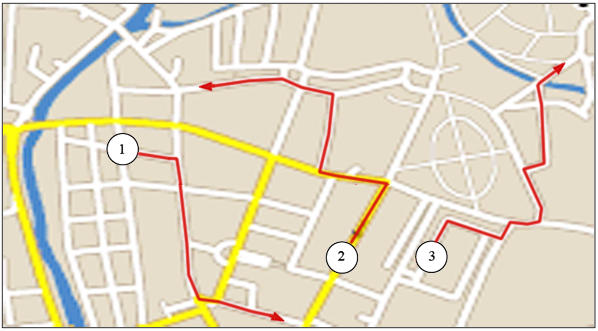
\includegraphics[scale=0.6]{4-movimento/img/waypoint_map.png}
    \caption{Example topography for Shortest Path Map-Based Movement Model}    
    \label{fig:waypoint_map}
  \end{center}
\end{figure}

\section{Routed Map-Based Movement}
A movement model in which nodes movements are completely determined is Routed Map-Based Movement (RMBM). In this model nodes move following predetermined routes, for the duration of the simulation (\figurename~\ref{fig:route_map}). Nodes adopting this model can easily emulate the scheduled and repetitive movement of public transport, e.g. buses, trams or trains.
\begin{figure}[!htpb]
  \begin{center}
    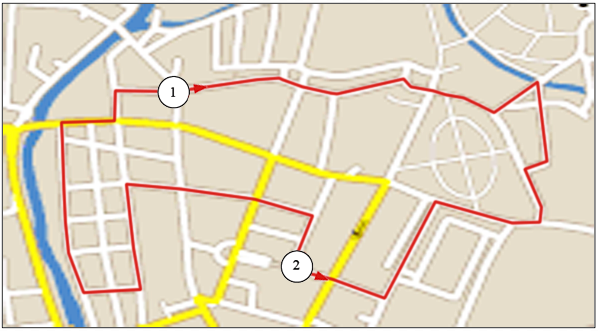
\includegraphics[scale=0.6]{4-movimento/img/route_map.png}
    \caption{Example topography for Routed Map-Based Movement Model}    
    \label{fig:route_map}
  \end{center}
\end{figure}

\section{Working Day Movement Model}
\label{descrWDM}
Movement models previously described are simple to understand and implement, but they don't capture completely such characteristics like heterogeneous behaviour, relationships between users or repetitive behaviour. Working Day Movement Model (WDM) \cite{articoloWdm} does this using a simple idea: people follow certain routines during a typical working day, e.g. going to work, going out with friends, etc. All these actions mean a person usually meets the same group of people. This reflects heterogeneity in user movement, i.e. one node will hardly ever meet all the other nodes in the simulation. This also raises locality in nodes movement, reducing encounters between nodes.
\\

During a typical working day simulated by this model, a node is involved in three main activities:
\begin{itemize}
\item sleep at home
\item work in the office
\item go out in the evening with friends
\end{itemize}
These activities can obviously vary from person to person, depending on the lifestyle of the subject. These are the most generic and can be associated to the typical working day of a great number of people.
\\

A person usually does these activities in the same locations, i.e. he sleep at home and works in the same office every day. It can be assumed that when he goes out with friends, they will go to a set of favourite places. These activities are repetitive, day after day, and are performed in places in common with other people. Simulating this, allows the spontaneous creation of user communities, e.g. people living in the same home location are a family, users working in the same office are colleagues and friends will meet to go together to their favourite places in the evening. A movement model able to emulate all these behaviours is fundamental to evaluate a protocol like M2MShare, where the frequency of encounters between nodes influences the routing strategy.\\

Creation of such communities of users, and in general relationships between nodes, are not shown using simpler movement models like RMBM or SPMBM i.e. in a longer period of time, each node is equally likely to meet any other node an equal number of times. In the Random Walk movement model, nearby nodes are more likely to come into contact and there are no clear relationships between nodes in most of the simpler models.
\\

To emulate the three main activities, WDM uses simpler mobility models as submodels. A node moving using WDM, will change several submodels during a single simulated day. Submodels are also used to simulate different modes used by nodes to move through the map. So, a person can move from one location to another by walking, driving his car (if it has one) or using public transport.
\\
%Per la simulazione delle attività giornaliere, WDM utilizza dei sottomodelli dedicati, oltre a dei sottomodelli preposti a simulare gli spostamenti fra un'attività e l'altra. Una persona si potrà quindi spostare a piedi, in auto o utilizzando i mezzi pubblici, a seconda della propria disponibilità e convenienza. Il fatto di muoversi da soli o in gruppo (prendendo lo stesso bus o camminando assieme la sera) permette di avere dei comportamenti eterogenei e quindi migliorare ulteriormente la realisticità degli spostamenti compiuti dai vari nodi.


\subsection{Example of working day}
During one typical working day, the starting location of a node is its own house. Every node has a wake up time, indicating what time that node leaves home in the morning. The value is drawn from a normal distribution with mean 0 and standard deviation configurable. The wake up time value is generated at the beginning of the simulation and remains the same for the duration of the simulation, i.e. every node leaves home at same time every day. Different values between nodes emulate differences in lifestyles, e.g. one person can get dressed faster in the morning and another can be slower.
\\ 

When a node leaves home, it travels to its destination, its office. This can be done by walking, driving its own car (if available) or using public transport. The choice of transportation is made by evaluating availability and speed of reaching the destination. The relative mobility submodel is used according to the chosen transportation.
\\

Once the node reaches its office, it stays there for the entire working time, which is a configurable value. After working hours, the node decides, by drawing, whether it returns home or goes out for the evening activity. Again, different submodels are used for transitions between the locations.


\subsection{Home Activity Submodel}
Every node has one location in the map set as Home Location. Home location is randomly chosen, for every node, at the beginning of the simulation between a set of geographical points in the related district of the map. The chosen location remains the same for the entire simulation duration, i.e. every node wakes up in the morning and returns in the evening to the same location.
\\

When the node returns home it moves near this location for a while and then it stays still until next wake up time. This behaviour is not an error, but it is done to emulate the activity of a mobile phone left in the same place inside the house while the user does typical domestic activities which do not involve the use of a mobile phone, e.g cooking, watching TV or sleeping.

\subsection{Office Activity Submodel}
The submodel related to the working activities is a model which emulates the behaviour of an employee inside the office. During the working time the employee stays at his desk for most of the time but it can leave it to attend a meeting, talk with a colleague or have a break. During all these moments it can meet nodes related to other colleagues.
\\

The office is described as a single room with rectangular shape, where the only entrance point, the door, is placed in the upper left hand corner. Every employee has its own desk, located in the same place inside the office for the duration of the simulation. In this model the presence of walls or other furniture inside the office is not simulated. To compensate for this, the office is described as a room larger than the normal size, to emulate the time needed to avoid obstacles and reach a destination when moving inside the office.
\\

When entered in the office, the employee moves directly to its desk and then stays there for an amount of time drawn from a Pareto distribution. When this period is passed, the node chooses a random destination inside the office, walks to reach it and then waits for an amount of time drawn from the same Pareto distribution, before returning to his desk. The repetition of these movements and pauses from the desk to some random location inside the office continues until working time expires. 
\\

The length of working time is a configurable parameter, as are configurable the distribution parameters. This allow to tune movements inside the office as there are a variety of different jobs and buildings where people move according to different patterns e.g. a teacher who moves every hour to change class inside a school or a cashier who does not leave her place at all during working time.


\subsection{Evening Activity Submodel}
The Evening Activity Submodel emulates activities performed after work, in the late afternoon or in the evening, like shopping, going eat in a restaurant or in a pizzeria. These activities are performed in group and with a configurable probability which determines if a person returns directly home after work, or stays out with friends.
\\

When working time is over, the node moves to one of its favourite places using one transport submodel. When arrived, it waits for other people until there are enough people to create a group and start the activity. The minimum number of people needed to create a group is configurable and when all groups for a place are full and a new person arrives, a new group is created.
\\

When a group is full, all people in the group walk together to reach a nearby, randomly chosen, location and they wait for a random amount of time, drawn from a range of values. This waiting time emulates the duration of the dinner, shopping or a movie at cinema and when it is over all nodes belonging to the group leave each other and return to their own houses.

\subsection{Transport Activity Submodel}
Transport Activity Submodels are used by nodes to move between home, office and evening activities.
\\

At the beginning of the simulation, a car is assigned to every node with configurable probability. Nodes with cars move always using it, while people who do not have one walk or use public transport. A model which uses different types of transport models adds additional heterogeneity and this also influences also routing protocols, since quicker nodes, like ones using cars for instance, can quickly transfer packets for longer distances.
\\

According to the chosen transportation, Transport Activity Submodel uses three different submodels:
\\

\begin{description}
\item [Walking Submodel]: nodes which do not have a car walk on the streets towards the destination at constant speed. They uses Dijkstra algorithm to find the shortest path from the current position to the destination.

\item [Car Submodel]: nodes with a car move faster than walking nodes, driving between one main activity and the next one, but walking during a single activities, i.e. they do not use the car inside the office, of course. In this model every car carries one single person and traffic congestion and traffic lights are not considered.

\item [Bus Submodel]: there can be several routes of public transport (buses, trams, trains) on the simulated map. Each route is run by several public transport according to a schedule. Each public transports can carry more than one person at a time.
\end{description}

Every person who does not have a car knows one bus route and can use every bus running on that route. The choice between walking or using public transport is done considering a difference between Euclidean distances. If the distance between node's location and the nearest bus stop summed with the Euclidean distance from the destination to the nearest bus stop is shorter than the Euclidean distance between the node's location and the destination, then the node uses the public transport system, otherwise it walks to the destination. If public transport is chosen the node changes between two transport submodels: it walks to the nearest bus stop using the Walking Submodel and then switches to the Bus Submodel, waiting for the bus. When the bus arrives, the node enters it and travels until to the bus stop closer to the destination. Finally it switches back to the Walking Submodel to reach the destination.
 
 
\section{Our choice}
To evaluate M2MShare performance in a realistic environment we use the Working Day Movement model in our simulations. While other simpler models can reproduce some characteristics in common with real traces, like contact and inter-contact times, they are not able to completely show human relationships and group movements between users. In \cite{Natarajan:2007:UUI:1762888.1762904} it is shown that analysing data from real traces, there appears a specific behaviour of users clustering in groups. 
\\

Two other aspects of human movement patterns are locality and heterogeneity. Locality is the tendency of nodes spending most of their time within a small area, so in a movement model with high locality, node's movement is restricted to a small portion of the simulated world. Heterogeneity implies differences in movement patterns and properties between nodes. These two aspects are not shown using simpler mobility models, like Random Walk or Random Waypoint, in which nodes have low locality (they move randomly through the whole area) and heterogeneity (they moves adopting the same behaviour for all the simulation, entering in contact with all other nodes with equal probability). In WDM locality is achieved assigning nodes to different home, office and evening activity locations. Heterogeneity is achieved using different transportations to move through the simulation area and using different distributions from which draw waiting times related to activities performed during the day.
\\

In M2MShare the creation of social relationships and spontaneous communities is very important and WDM is able to show such human behaviours in its way of emulating daily activities performed by a user in places common to other users. This ability is very useful to realistically move nodes emulating M2MShare users and it is one of the main reasons why we chose WDM for our simulations.
\\

Finally, WDM is very configurable and this is another important characteristic because it is practical to have a model with configurable parameters to work with, especially to test how a protocol like M2MShare performs when certain parameters change, to better be able to discover weaknesses and strengths.
 
%In M2MShare we saw that nodes movement is used to extend the search area for a requested file, delegation of unaccomplished tasks are done to servant nodes exploring different areas and frequency of encounters between nodes are used to determine if a node can be a good servant to delegate to it a task.

%It is also practical to have a model with configurable parameters to work with. Sometimes a protocol or an application developer wants to test how the protocol or application performs when certain parameters change, to better be able to find out weaknesses and strengths. Sometimes researchers also need a very simple model to work with, to be able to use it in mathematical proofs for various theorems.

%Synthetic models are often preferred since they are easier to work with than real user traces. Moreover, real user traces are rarely available for the environment to be modelled. Additionally, researchers want to do sensitivity analysis to find out how protocols and applications perform under different conditions. This is not possible with real user traces unless a parameterized model has been successfully extracted. 


%Hsu and Helmy [26] show by studying real user traces that nodes are very often turned on/off and only visit a small portion of the WLAN access points in campus areas. Moreover, they find that node mobility while using network is very low and one node only meets a small portion of all other nodes in the area. These types of characteristics are usually not captured in movement models. Furthermore, they reveal repetitive patterns with a period of one day and heterogeneity among nodes. Although heterogeneity and repetitiveness has been modeled, most simple movement models do not. According to Hsu and Helmy, the biggest issue with most synthetic models is that they are not capturing such characteristics as heterogeneous behavior, switching devices on/off or relationships between users. We noticed that even though most of the known features of movement have been modeled, no model exist where all or many of the features have been combined. Our approach is to combine these different elements to create a new movement model.

% ---------------------------------------------------------------------------
%: ----------------------- end of thesis sub-document ------------------------
% ---------------------------------------------------------------------------

